\chapter{The LHCb experiment}
\label{cap:LHCb}

\section{The Large Hadron Collider}

\begin{figure}[t]
	\centering
	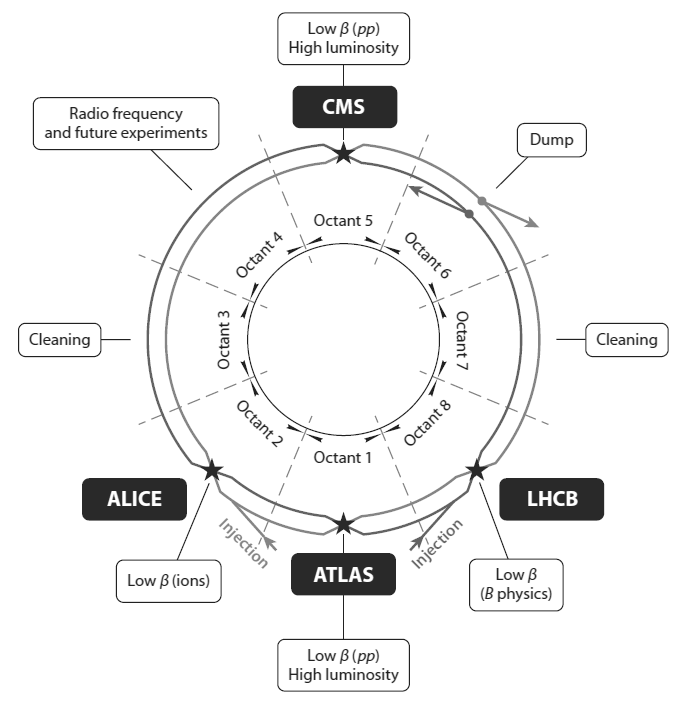
\includegraphics[width=.6\textwidth]{graphics/02-lhcb/lhc_diagram.png}
	\caption[LHC schematic layout.]{Layout of the Large Hadron Collider with its four main experiments \cite{doi:10.1146/annurev-nucl-102010-130438}.}
	\label{fig:2:lhc_diagram}
\end{figure}

At the moment of writing, the Large Hadron Collider (LHC for short) is the largest and most powerful particle collider in the world.
When the LHC was first approved by the European Organization for Nuclear Research (CERN) in 1994, it was originally going to be built with an initial center-of-mass collision energy of \SI{10}{\tev}, with the plan to upgrade it to \SI{14}{\tev} at a later stage;
however, after negotiations with nonmember states, in 1996 the CERN council approved the construction at \SI{14}{\tev} energy in one stage \cite{doi:10.1146/annurev-nucl-102010-130438}.
First collisions were obtained in 2010 at center-of-mass energy of \SI{7}{\tev}, with the current world record of \SI{13}{\tev} being achieved in 2015 after the first Long Shutdown.

LHC is located at the CERN laboratory near Geneva, Switzerland, housed in the underground tunnel previously occupied by the LEP experiment.
Its structure, sketched in Figure \ref{fig:2:lhc_diagram}, consists of two counterrotating rings hosting beams for particle-particle collisions (mainly protons, but LHC is also used for ion collisions).

Four main experiments are stationed at the LHC ring intersection points:
ATLAS and CMS are high-luminosity experiments focused on general purpose proton-proton collisions; ALICE is optimized for lead-on-lead collisions with lower center-of-mass energy and luminosity compared to the former two; finally, LHCb is dedicated on the study of $b$ hadrons and will be the focus of the rest of this Chapter.
Beyond the above four, a number of small-scale, more specialized experiments also work with LHC, such as TOTEM, MilliQan and MoEDAL.

Broadly speaking, the LHC schedule alternates data taking periods (\textit{Runs}) with maintenance work periods (\textit{Long Shutdowns}, LS for short);
while the shutdowns are designed for consolidation and improvement of the collider itself, mainstay experiments usually take advantage of the hiatus to upgrade their detectors both in hardware and software.

@todo: discussione delle Run.


\section{The LHCb experiment and detector}

\begin{figure}[t]
	\centering
	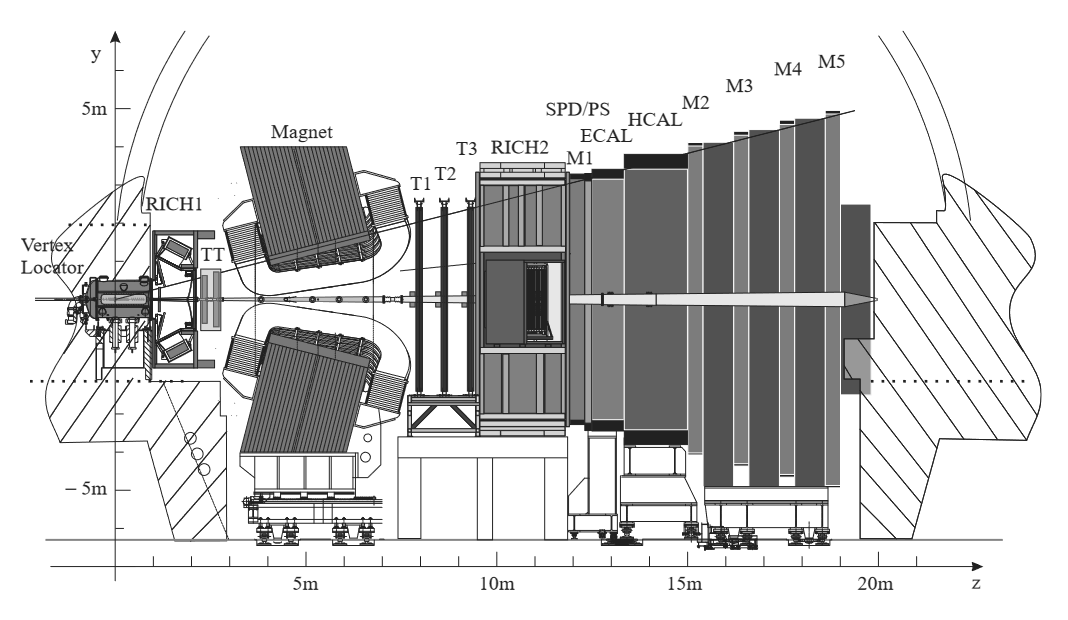
\includegraphics[width=\textwidth]{graphics/02-lhcb/lhcb_diagram.png}
	\caption[LHCb detector side view.]{Side view (bending plane) of the LHCb detector used for LHC Runs 1 and 2 \cite{Antunes-Nobrega:630827}.}
	\label{fig:2:lhcb_diagram}
\end{figure}

LHCb (the \textit{b} stands for \textit{beauty}\footnote{Before settling on the names \textit{top} and \textit{bottom} for the third generation of quarks, the names \textit{truth} and \textit{beauty} were among those proposed. While they never gained enough momentum in the scientific community, echoes of the failed nomenclature are still present in heavy quark vocabulary, for instance in the alternative name \textit{truth} for the \textit{topness} flavour number mentioned in Section \ref{sec:flavour-physics}, as well as in the official name for the LHCb experiment.}) is a single-arm detector designed to study heavy-flavour physics at the LHC, with the main objective of providing precision measurements of CP violation and rare decays of $b$ and $c$ hadrons \cite{Alves:1129809}.

Unlike the other three main experiments at LHC, LHCb has a forward-optimized geometry shown in Figure \ref{fig:2:lhcb_diagram}, with an angular acceptance of $10\div300$ \si{\mrad} in the bending plane and $10\div250$ \si{\mrad} in the non-bending plane\footnote{For the sake of brevity, I'll refer to it as the 300/250 \si{\mrad} acceptance.}.
Such a layout, more reminiscent of fixed target experiments than beam colliders, is motivated by the fact that $b\bar{b}$ pairs produced at high energies are usually collimated in the same forward/backward cone.
A more in-depth look at the tracking and particle identification systems will be taken in Sections \ref{sec:2:tracking} and \ref{sec:2:pid} respectively.
\label{info:LHCb_system}
The standard LHCb coordinate system, used as reference for the rest of this thesis, is a right-handed system centered on the beam interaction point, with the $z$ axis along the the beam pipe and $y$ axis directed vertically upwards.

Elenca i successi.

\subsection{Tracking}
\label{sec:2:tracking}
In order to measure the momenta of charged particles through their bending curve, LHCb employs a dipole magnet \cite{Amato:424338} consisting of two trapezoidal coils bent at $45^\circ$ on the two transverse sides, seen in Figure \ref{fig:2:lhcb_diagram} around $z\approx \SI{5}{\meter}$ (the magnet is placed so that the line connecting the centers of the pole faces crosses $z=\SI{5.3}{\meter}$).

\begin{figure}[t]
	\centering
	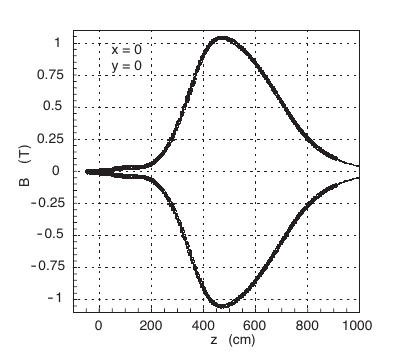
\includegraphics[width=.6\textwidth]{graphics/02-lhcb/b_field_map_z.png}
	\caption[LHCb magnetic field along the $z$ axis.]{LHCb magnetic field along the $z$ axis \cite{Amato:424338}.}
	\label{fig:2:b_field_map_z}
\end{figure}

This magnet provides an integrated field of $\int B dl \approx \pm \SI{4}{\tesla\meter}$ for \SI{10}{\meter} tracks\footnote{The $\pm$ sign is due to the fact that the magnet operates alternatively in up and down polarities, inverting the sign of the magnetic field.}.
Most of this field is contained in the $z\in[2.5,7.95]$ \si{\meter} region, with 
a small fraction ($\int B dl \approx \SI{0.12}{\tesla\meter}$) upstream of $z=\SI{2.5}{\meter}$. The field map along $z$, measured with a precision of $4 \times {10}^{-4}$, is shown in Figure \ref{fig:2:b_field_map_z} for $x=y=0$.
Dishomogeneities in the $xy$ plane for fixed $z$ are estimated at $\lesssim 6\%$ within the LHCb detector acceptance.

\subsubsection{VELO}
As the name suggests, the VErtex LOcator (VELO) system \cite{Barbosa-Marinho:504321} is designed to provide precision measurements of charged tracks near the beam interaction point, in order to correctly reconstruct detached secondary vertices typical of $b$- and $c$-hadron decays.

\begin{figure}[t]
	\centering
	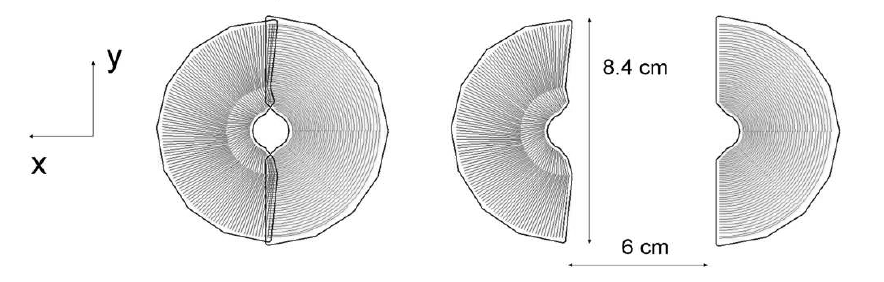
\includegraphics[width=\textwidth]{graphics/02-lhcb/VELO_xy.png}
	\caption[Front view diagram of the VELO detector.]{Front view diagram of the VELO detector in fully closed (\textit{left}) and fully open (\textit{right}) configurations \cite{Barbosa-Marinho:504321}.}
	\label{fig:2:VELO_xy}
\end{figure}

The VELO detector comprises 42 silicon modules along the beam direction, each consisting of a pair of half discs measuring the radial and azimuthal track coordinates respectively. These modules cover the $1.6 < \eta < 4.9$ positive pseudorapidity range, as well as some negative pseudorapidity portion to improve primary vertex reconstruction, and are able to detect particles emerging from primary vertices with $|z| < \SI{10.6}{\centi\meter}$.
Due to high risk of radiation damage during beam injection from the Super Proton Synchrotron (SPS) into LHC, these modules can be retracted by \SI{3}{\centi\meter} in so-called \textit{fully open} configuration, whereas during collision phase the VELO operates in \textit{fully closed} configuration (see Figure \ref{fig:2:VELO_xy}).

\begin{figure}[t]
	\centering
	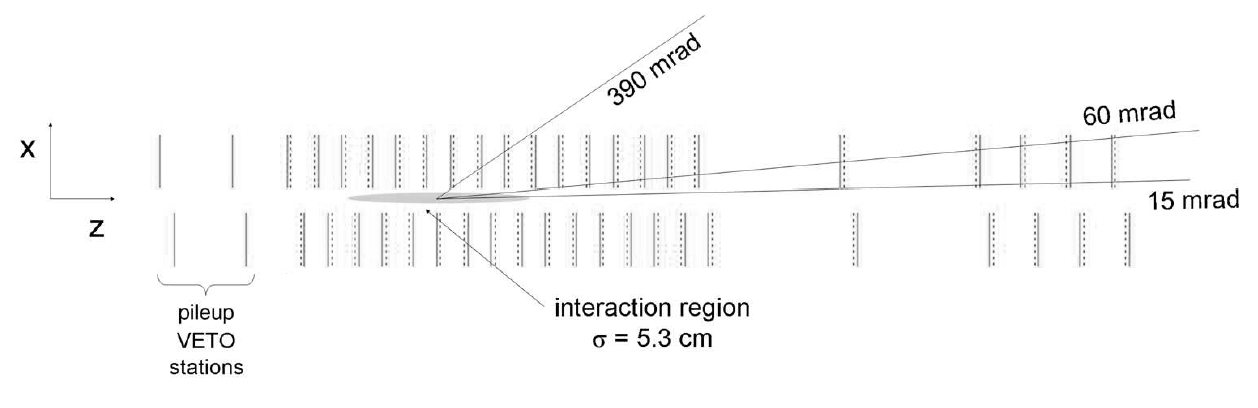
\includegraphics[width=\textwidth]{graphics/02-lhcb/VELO_xz.png}
	\caption[Cross section diagram of the VELO detector in the $xz$ plane.]{Cross section diagram of the fully closed VELO detector in the $xz$ plane at $y=0$ (top view). Radial sensors are depicted as \textit{solid} segments, azimuthal sensors as \textit{dashed} segments \cite{Barbosa-Marinho:504321}.}
	\label{fig:2:VELO_xz}
\end{figure}

Figure \ref{fig:2:VELO_xz} shows the $xz$ plane cross section of the VELO modules; the two halves of the detector are $z$-shifted by \SI{1.5}{\centi\meter} to ensure full azimuthal acceptance, resulting in the partial overlap seen in fully closed configuration.
Four radial-only \textit{pile-up sensors}, part of the Level-0 hardware trigger system (see Section \ref{sec:2:data_flow}), are placed upstream to help veto multiple-interaction events.



\subsubsection{Tracker Turicensis}
The Tracker Turicensis (TT) \cite{Gassner:728548}, formerly known as Trigger Tracker, is a $\SI{150}{\centi\meter} \times \SI{130}{\centi\meter}$ tracking station located just upstream of the dipole magnet.
Its placement serves the main purpose of tracking low-momentum particles ($|\vec{p}| \lesssim \SI{1.5}{\gev\per c}$) that would otherwise be bent out of the detector by the magnet without reaching the T stations.

The TT consists of four readout layers of silicon microstrip sensors arranged in a $x$-$u$-$v$-$x$ configuration (vertical in the first and last layers, rotated by a stereo angle of $\mp 5^\circ$ in the second and third layer respectively) for a total active area of $\approx \SI{8.4}{\meter\squared}$.
A \SI{200}{\micro\meter} strip pitch ensures a single-hit resolution $\lesssim \SI{50}{\micro\meter}$.

\begin{figure}[t]
	\centering
	\includegraphics[width=.6\textwidth]{graphics/02-lhcb/TT_layout.png}
	\caption[Front view of the third TT layer.]{Front view of the third TT layer (different readout sectors are labeled with different shadings) \cite{Alves:1129809}.}
	\label{fig:2:TT}
\end{figure}

The third TT layer is depicted in front view in Figure \ref{fig:2:TT}.
The basic unit of a layer is the \textit{half module}, covering half the LHCb height acceptance.
Each half module consists of a row of seven sensors bonded together to form either three or two \textit{readout sectors}.
Modules near the beam pipe are of the former category, with four sensors bonded in the L sector, two in the intermediate M sector and a single sensor for the K sector closest to the beam ($4$--$2$--$1$ modules);
other modules forgo the K sector and bond the spare sensor in the M sector ($4$--$3$ modules).
Front-end readout hybrids, one for each sector, are placed at the L-end of the half modules, outside of the detector acceptance, connected directly to the L sector and indirectly to the M and K sectors via Kapton flex cables.

\subsubsection{T stations}
\begin{figure}[t]
	\centering
	\begin{subfigure}{.45\textwidth}
		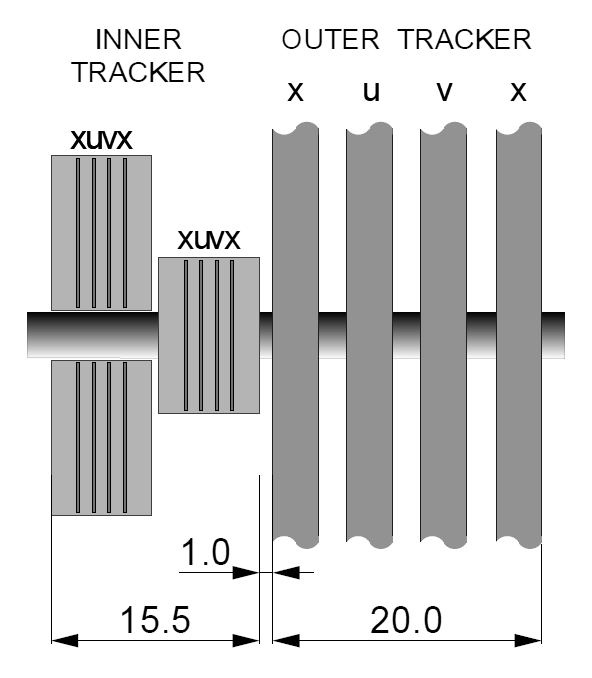
\includegraphics[width=\textwidth]{graphics/02-lhcb/t_station_top_view.png}
		\caption{}
		\label{fig:2:t_station_top}
	\end{subfigure}
	\begin{subfigure}{.45\textwidth}
		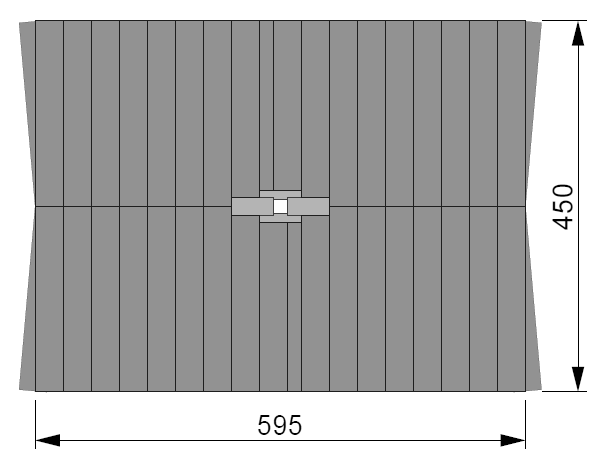
\includegraphics[width=\textwidth]{graphics/02-lhcb/t_station_front_view.png}
		\caption{}
		\label{fig:2:t_station_front}
	\end{subfigure}
	\caption[Top and front views of a T tracking station.]{Top (\textit{left}) and front (\textit{right}) views of a T tracking station \cite{Barbosa-Marinho:582793}. IT and OT are labeled with lighter and darker shades of grey respectively. Dimensions are given in \si{\centi\meter}; for the top view, lateral dimensions are not to scale.}
	\label{fig:2:t_station}
\end{figure}

The three T stations, labeled as T1--3, are the last line of defense for LHCb tracking purposes, covering the $z \approx 7.7 \div 9.4\,\si{\meter}$ region downstream of the dipole magnet \cite{Barbosa-Marinho:582793}.
Each T station is composed of an Inner Tracker for the region near the beam pipe and an Outer Tracker for the outer regions, as sketched in Figure \ref{fig:2:t_station}.

\begin{figure}[t]
	\centering
	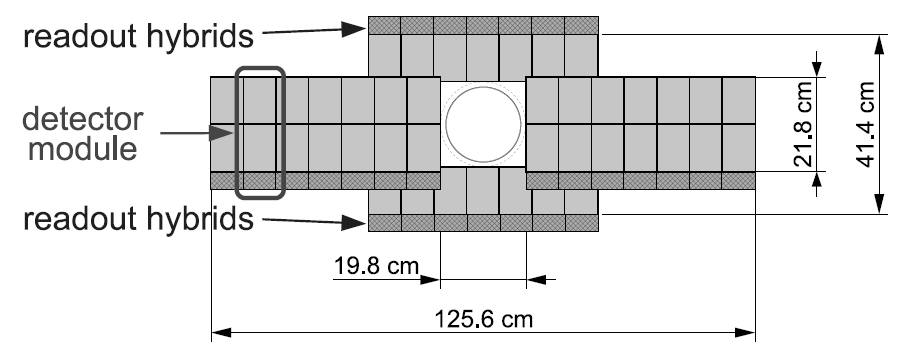
\includegraphics[width=.6\textwidth]{graphics/02-lhcb/it_layout.png}
	\caption[Front view of an Inner Tracker $x$ layer.]{Front view of an $x$ detector layer in the T2 Inner Tracker \cite{Alves:1129809}.}
	\label{fig:2:IT}
\end{figure}

The Inner Tracker (IT) \cite{Barbosa-Marinho:582793} shares many similarities with the TT design, being developed in conjuction with it under the common Silicon Tracker (ST) project.
Sporting the same four layers of silicon microstrips in $x$-$u$-$v$-$x$ configuration, it covers a comparably smaller $\SI{120}{\centi\meter} \times \SI{40}{\centi\meter}$ cross-shaped surface (see Figure \ref{fig:2:IT}) for a total active area of $\approx \SI{4}{\meter\squared}$, less than half the TT.
As a consequence, individual modules only include one or two sensors  connected to the readout hybrids via a pitch adapter.

By contrast, the much larger Outer Tracker (OT) \cite{Barbosa-Marinho:519146} is a drift detector consisting in an array of Ar/CO$_2$ straw-tube modules.
Each module contains two layers of straw tubes with \SI{4.9}{\milli\meter} inner diameter, ensuring a \SI{50}{\nano\second} drift time and \SI{200}{\micro\meter} spatial resolution.
Within a single T station, said modules are arranged in four layers in $x$-$u$-$v$-$x$ configuration (see Figure \ref{fig:2:t_station_top}) with $\pm 5^\circ$ vertical tilt for $u$ and $v$ layers respectively.
The OT covers the entire 300/250 \si{\milli\rad} LHCb detector acceptance.

\subsubsection{Track classification and the problems with T tracks}
Overall, the LHCb tracking system has very high efficiency, besting $96\%$ in the momentum range $|\vec{p}| \in \left[5, 200\right]$ \si{\gev\per c} for tracks crossing all three detector stations (VELO, TT and T1--3). \cite{HistoryLHCb}
However, not all particles enjoy this luxury:
low momentum particles ($|\vec{p}| \lesssim \SI{1.5}{\gev\per c}$) are unable to reach the T stations due to the sharp magnet bending curve, while daughters of longer-lived particles with $c\tau \gtrsim \SI{30}{\centi\meter}$ will miss the VELO and possibly even the TT detector.

\begin{figure}[t]
	\centering
	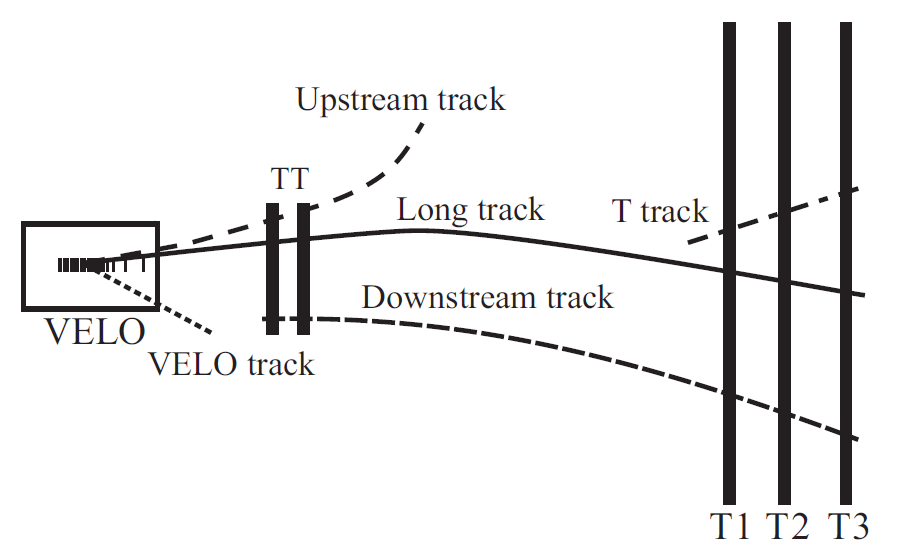
\includegraphics[width=.8\textwidth]{graphics/02-lhcb/Track_Definitions.png}
	\caption[Side view diagram of LHCb tracking system and track categories.]{Side view diagram of the LHCb tracking systems for LHC Runs 1 and 2 with sketched examples of the main track classification categories.}
	\label{fig:2:track_classification}
\end{figure}

Thus, in spite of the great efficiency, it's useful to define track categories in the LHCb working environment depending on what hits were recorded in which detectors:
\begin{itemize}
	\item \textit{Long} tracks
	\item \textit{Upstream} tracks
	\item \textit{Downstream} tracks
	\item \textit{T} tracks
\end{itemize}
Sketches of tracks satisfying the above requirements are depicted in Figure \ref{fig:2:track_classification}.

@todo: \textbf{tutta} la storia delle T track. Le prime slide delle presentazioni, in pratica.

\subsection{Particle identification}
\label{sec:2:pid}
While tracking outgoing particles is obviously of paramount importance for physics analysis, knowledge of \textit{what} particles are being tracked is also crucial.
The ability to distinguish protons, pions and kaons is of particular interest at LHCb due to its research objectives in CP violation and $b$ physics, requiring precise flavour tagging and physical background rejection.
For the above reasons, a complex ecosystem of detectors dedicated to particle identification (PID) is in place.

\subsubsection{RICH}
Roughly $90\%$ of pions, protons and kaons from $B$ meson decays have momentum in the $[2,150]$ \si{\gev\per c} range \cite{HistoryLHCb}.
Since the momentum spectrum changes at different polar angles, LHCb employs two Ring Imaging CHerenkov (RICH) detectors \cite{Amato:494263} to cover the full momentum range for these particles.

\begin{figure}[t]
	\centering
	\begin{subfigure}{.45\textwidth}
		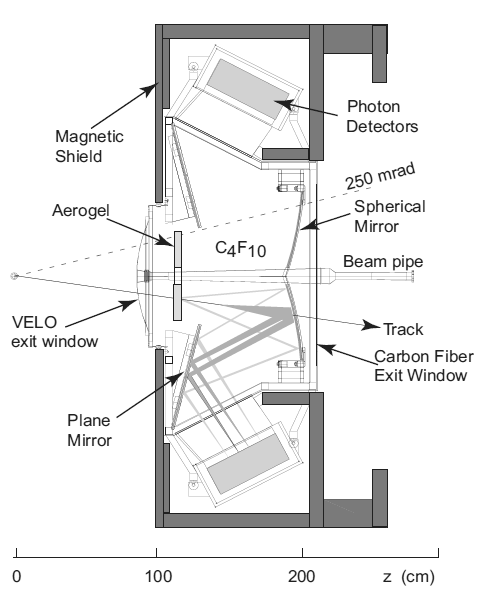
\includegraphics[height=.3\textheight]{graphics/02-lhcb/rich1_top.png}
		\caption{}
		\label{fig:2:rich_1_top}
	\end{subfigure}
	\begin{subfigure}{.45\textwidth}
		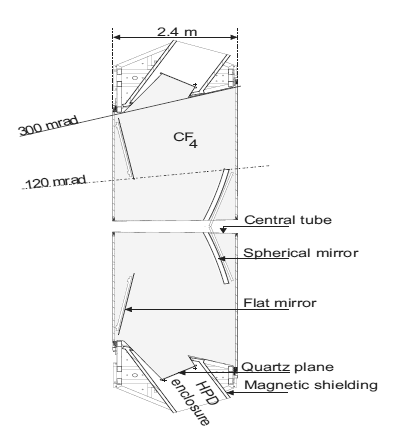
\includegraphics[height=.3\textheight]{graphics/02-lhcb/rich2_top.png}
		\caption{}
		\label{fig:2:rich_2_top}
	\end{subfigure}
	\caption[Top view of the two RICH detectors.]{Top view of the RICH 1 (\textit{left}) and RICH 2 (\textit{right}) detectors \cite{Alves:1129809}.}
	\label{fig:2:rich_top}
\end{figure}

The RICH 1 detector, sketched in Figure \ref{fig:2:rich_1_top}, is located upstream of the dipole magnet, wedged between the VELO and TT tracking detectors.
The detector exploits the different spectra of Cherenkov angles as a function of momentum for different kinds of particles.
At the beginning of Run 1, RICH 1 used two radiator materials: an aerogel layer ($n=1.03$) and a C$_4$F$_{10}$ gas layer ($n=1.0014$).
This allowed RICH 1 to perform $\pi/K$ identification in the $1\div 60$ \si{\gev\per c} range.
Due to occupancy problems, the silica aerogel radiator providing identification in the low momentum range $|\vec{p}| \lesssim \SI{10}{\gev\per c}$ was removed for Run 2;
since the kaon Cherenkov threshold in C$_4$F$_{10}$ is $\approx \SI{9.7}{\gev\per c}$, they can still be identified by operating RICH in so-called \textit{kaon veto mode}, i.e. 
by the lack of Cherenkov light \cite{HistoryLHCb} \cite{RichPerformance}.
RICH 1 covers from $\SI{25}{\mrad}$ (lower limit imposed by the beryllium beam pipe section) up to the full 300/250 \si{\mrad} LHCb acceptance.

Acting as complement to its partner, RICH 2 (Figure \ref{fig:2:rich_2_top}) operates downstream of the T tracking stations and is optimized for a high momentum range, providing PID from $\approx \SI{15}{\gev\per c}$ up to and beyond $\SI{100}{\gev\per c}$.
Its lower limit of acceptance is $\approx \SI{15}{\mrad}$, dictated by the required clearance of \SI{45}{\milli\meter} around the beam pipe.

\subsubsection{Calorimeter}
The LHCb calorimeter system \cite{Amato:494264} serves the dual purpose of identifying hadrons, electrons and photons and measuring their energies.

\subsubsection{Muon system}

\section{The LHCb data flow}
\label{sec:2:data_flow}
\begin{figure}[t]
	\centering
	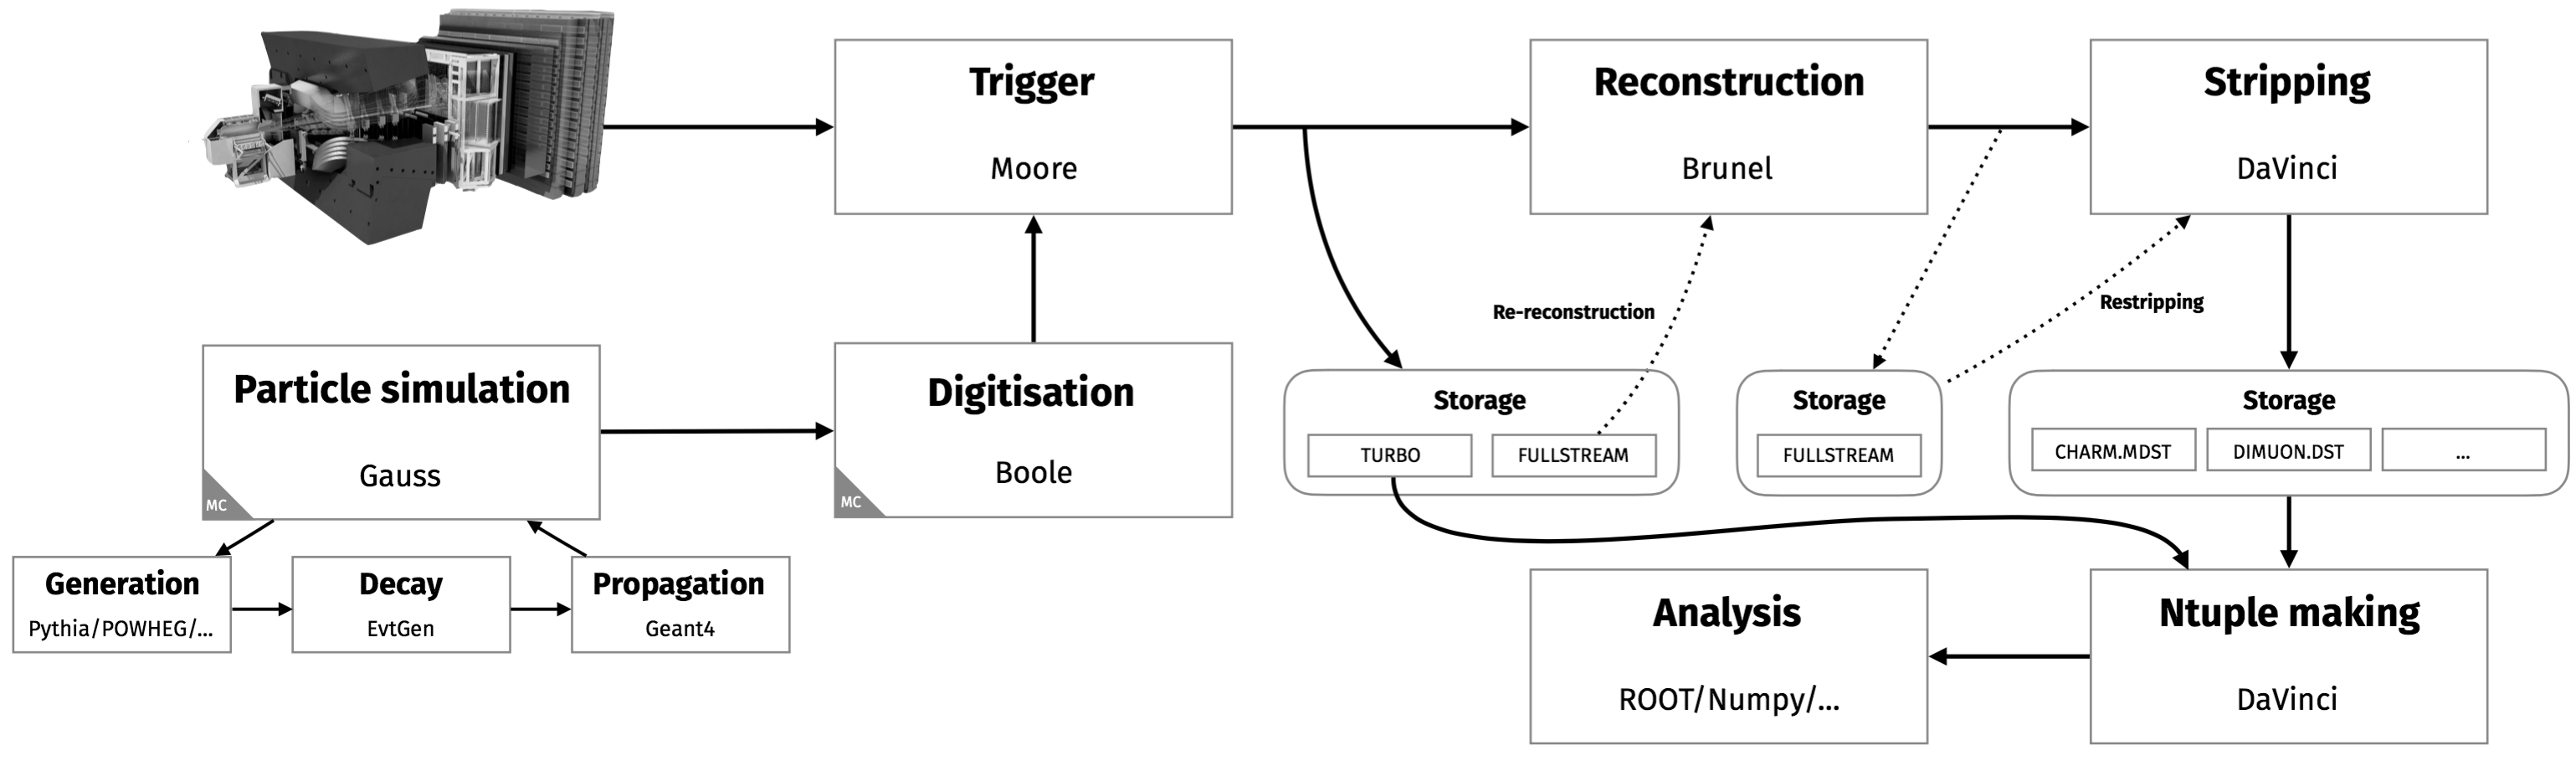
\includegraphics[width=\textwidth]{graphics/02-lhcb/lhcb_run_2_data_flow.png}
	\caption{Diagram of the LHCb Run 2 data flow.}
	\label{fig:2:lhcb_data_flow}
\end{figure}

Qui trigger, track reconstruction e tutto il resto.

\section{LHCb detector upgrade for Run 3}

\begin{figure}[t]
	\centering
	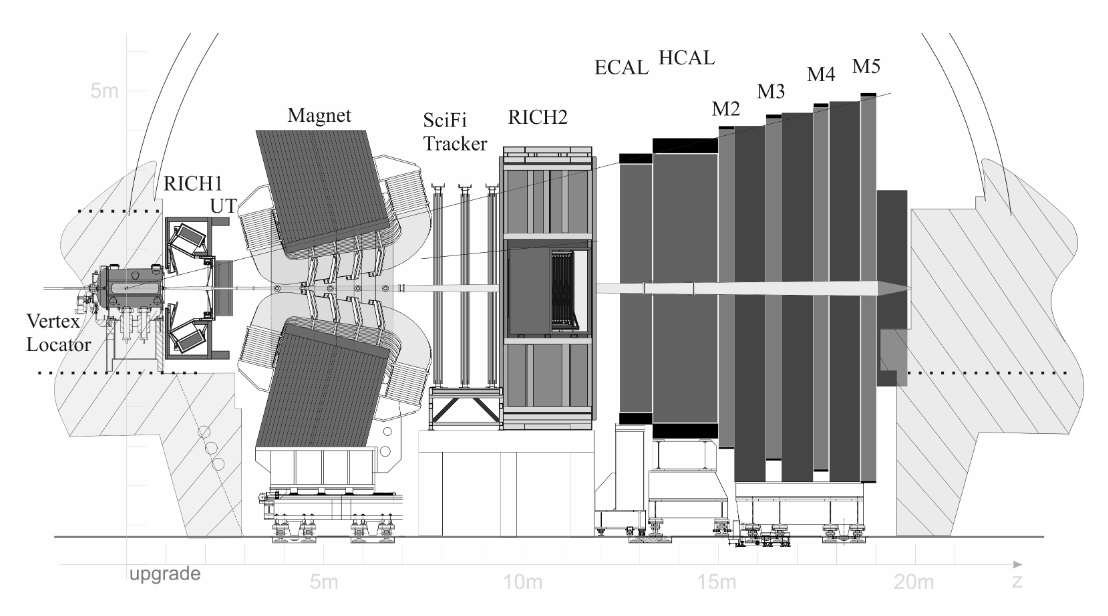
\includegraphics[width=\textwidth]{graphics/02-lhcb/lhcb_diagram_run3.png}
	\caption[LHCb detector side view.]{Side view (bending plane) of the upgraded LHCb detector for future usage in LHC Run 3 \cite{Piucci_2017}.}
	\label{fig:2:lhcb_diagram_run3}
\end{figure}

\section{Data}
Non so se vada qui ma da qualche parte deve andare.